	\chapter{CONTEO DE ESPECTROS SERIALES}
	\section{Espectros de las funciones \{I, T, R\}}
		\label{espec}		
		
		\begin{wrapfigure}{R}{0.25\textwidth}
			\captionsetup{justification=centering, font=footnotesize}
			\vspace{-0.5cm}
			\centering{
				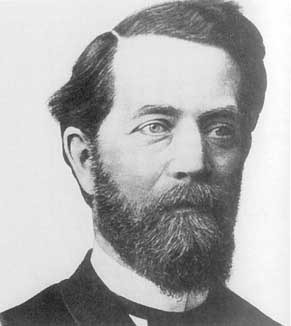
\includegraphics[width=0.22\textwidth]{Felix_Klein.jpeg}			
				\caption*{Felix Klein\\(1849--1925)}	}
			
			%\vspace{-0.5cm}
		\end{wrapfigure}
		Es interesante conocer el número de espectros seriales distintos que un compositor puede escoger. Al fin y al cabo, es irrelevante qué serie se escoge como la original dentro de su espectro serial, ya que produce el mismo material compositivo que cualquiera de su mismo espectro.
		
		Para calcular el número de espectros seriales se redefinirán las funciones transformativas para una longitud serial arbitraria, $n$, que será mayor que 2. Para $n=0,\ 1$ y 2 se realizará el cálculo en el apartado \ref{monodi}. 
	
		Además, como las transposiciones siempre son distintas entre sí, siempre pertenecen al mismo espectro. Se tomarán a partir de ahora todas ellas como equivalentes, de manera que solo se necesita hacer el cálculo para \{I, R\}.
		
		Al calcular con permutaciones se trabajará módulo $n$. La retrogradación sigue siendo R($\sigma(m))=\sigma(-1-m)$. La inversión será I($\sigma(m))=-\sigma(m)$, omitiendo la transposición habitual, ya que se toman las series transpuestas como equivalentes. De esta forma $-\sigma(m)+2\sigma(0)\equiv-\sigma(m)$. La retrogradación invertida es, por tanto, la composición de ambas: 
		
		RI($\sigma(m))=\text{I}\circ\text{R}(\sigma(m))=\text{I}\left(\text{R}(\sigma(m))\right)=-\sigma(-1-m)$.
		
		La retrogradación, la inversión y la composición de ambas cumplen que al aplicarlas dos veces se vuelve a la serie original. En teoría de grupos se diría que tienen orden 2. Entonces, \{Id, I, R, IR\} forma un grupo especial llamado \textit{grupo de Klein}, donde RI $\equiv$ IR, ya que estamos tomando las series transpuestas como equivalentes. 
		
		En general, un grupo de Klein es el formado por cuatro elementos donde cada elemento es inverso de sí mismo. El grupo de Klein, llamado así en honor al matemático alemán Felix Klein, es el grupo $\mathbb{Z}/(2)\times\mathbb{Z}/(2)$, producto directo de dos copias del grupo cíclico de orden 2.
		
		Por el lema de Burnside, explicado y demostrado en el apartado \ref{burnside}:	
		$$\#\text{Spec}=\#Orb=\frac{1}{|\mathbb{Z}/(2)\times\mathbb{Z}/(2)|}\sum_{\sigma\in\text{S}_n}|\text{Stab}(\sigma)|=\frac{1}{4}\sum_{\sigma\in\text{S}_n}|\text{Stab}(\sigma)|$$
		
		Es decir, se deben calcular para cada posible serie $\sigma\in\text{S}_n$ cuántas funciones transformativas lo dejan igual o equivalente bajo transposición.
		
		Como los estabilizadores son subgrupos, por el teorema de Lagrange su tamaño debe ser divisor del tamaño del grupo total. Entonces se pueden agrupar los estabilizadores por sus tamaños: 1, 2 o 4, y así calcular $\sum|\text{Stab}(\sigma)|$ agrupando todas las permutaciones con igual tamaño de estabilizador. Si $\#\sigma_i$ es el número de permutaciones cuyos estabilizadores tienen tamaño $i$:		
		$$\sum_{\sigma\in\text{S}_n}|\text{Stab}(\sigma)|=1\cdot(\#\sigma_1)+2\cdot(\#\sigma_2)+4\cdot(\#\sigma_4)$$
	
		Primero, se ha de ver que una permutación nunca va a ser igual ni equivalente mediante transposiciones a su inversa.	\label{inversano}	
		$$-\sigma(m)\equiv\sigma(m)\ \forall m\in \mathbb{Z} / (n) \implies 0\equiv2\sigma(m)\implies n\equiv2\sigma(m) \implies \frac{n}{2}\equiv\sigma(m)$$
		
		Así, $\sigma(m)$ sería constante para todo $m\in \mathbb{Z} / (n)$, lo cual es imposible. Esto implica que ninguna permutación va a tener a I en su estabilizador, por lo que $\#\sigma_4=0$. Queda entonces calcular cuántas permutaciones son equivalentes a su retrogradación y cuántas a su retrogradación inversa. La suma de ambas dará $\#\sigma_2$.
	
	\subsection{Elementos estables mediante R}
		Las permutaciones que coinciden con alguna transposición de su retrogradación cumplen, para $\gamma$ constante:
		$$\gamma+\sigma(m)=\text{R}(\sigma(m))=\sigma(-1-m)$$
		Aplicándolo a $(-1-m)$: $\qquad\gamma+\sigma(-1-m)=\sigma(-1-(-1-m))=\sigma(m)$
		
		De ambas ecuaciones: $\qquad\gamma=\sigma(-1-m)-\sigma(m)=\sigma(m)-\sigma(-1-m)$
		$$2\sigma(m)\equiv2\sigma(-1-m)\implies2\sigma(m)-2\sigma(-1-m)\equiv0$$	$$2\sigma(m)-2\sigma(-1-m)=n \implies \sigma(m)-\sigma(-1-m)=\frac{n}{2}$$
		Entonces $n$ debe ser par. Cuando $n$ es impar este tipo de permutaciones no existe. Además, cumplen que sus elementos simétricos se distancian entre sí un intervalo de $\frac{n}{2}$ unidades: son series con simetría par.
		$$\gamma=\sigma(m)-\sigma(-1-m)=\frac{n}{2}$$
		
		En una serie de longitud $n$, existen $\frac{n}{2}$ intervalos que miden $\frac{n}{2}$. Como no importa por cuál de ellos comience la serie, ya que las transportaciones son equivalentes, se fija el primero de los intervalos. Quedan los otros $\frac{n}{2}-1$ intervalos por escoger, así que el número de series con simetría par cuenta las permutaciones de $\frac{n}{2}-1$ intervalos y las dos posibles posiciones de cada intervalo -- creciente y decreciente --. \cite{reiner} Por ello, el número de series con simetría par es de:
		$$2! \cdot \left(\frac{n}{2}-1\right)! = 2\left(\frac{n-2}{2}\right)!=(n-2)(n-4)\ldots=(n-2)!!\ \footnote{Por definición, si $n$ es par $n!!=n(n-2)(n-4)\ldots4\cdot2$ y si $n$ es impar $n!!=n(n-2)(n-4)\ldots3\cdot1$.}$$

	\subsection{Elementos estables mediante RI}
		Las permutaciones que coinciden con alguna transposición de su retrogradación inversa cumplen, para un $\gamma$ constante:
		$$\sigma(m)=\text{RI}(\sigma(m))+\gamma=-\sigma(-1-m)+\gamma$$
		$$\gamma=\sigma(m)+\sigma(-1-m)$$
		
		Sus elementos simétricos suman una cantidad constante: son series con simetría impar. Tal y como se ha hecho en el apartado anterior, se puede fijar una de las notas, ya que las transportaciones son equivalentes. Si $n$ es impar, la nota central es $\sigma(\frac{n-1}{2})$, que es igual a $\sigma(-1-\frac{n-1}{2})$. Por tanto, $\gamma=2\cdot\sigma(\frac{n-1}{2})$. Si se escoge esta nota para ser fijada a 0, entonces $\gamma=2\cdot0=0$. Es decir, $\gamma$ puede ser fijada a 0 sin pérdida de generalidad.
		
		Para el resto de notas, $\sigma(m)=-\sigma(-1-m)$. Ya escogida la nota central, permite $n-1$ posibilidades para $\sigma(0)$. Ya escogidas la nota central, la primera y su simétrica, permiten $n-3$ posibilidades para $\sigma(1)$, y así sucesivamente hasta llegar a la nota anterior a la central, que es $\frac{n-3}{2}$. Por ello, para $n$ impar, el número de series con simetría impar es de:	
		$$(n-1)(n-3)\ldots(n-2\cdot\frac{n-5}{2}-1)(n-2\cdot\frac{n-3}{2}-1)=$$
		$$=(n-1)(n-3)\ldots(n-(n-5)-1)(n-(n-3)-1)=$$
		$$=(n-1)(n-3)\ldots4\cdot2=(n-1)!!$$
		
		Si $n$ es par, $\sigma(m)\neq\sigma(-1-m)\ \forall m\in \mathbb{Z} / (n)$, ya que no hay elemento central. Sea ahora $\gamma=2k$ un número par. Como $2k\leq n$ y las permutaciones son suprayectivas, para algún $m$ se cumple que $\sigma(m)=k$. Se tiene entonces $k+\sigma(-1-m)=2k\implies\sigma(-1-m)=k=\sigma(m)$. Como esto es una contradicción, $\gamma$ debe ser impar.
		
		Fijando, por ejemplo, $\sigma(0)=0$, se tienen $\frac{n}{2}$ posibilidades para $\sigma(-1-m)$, es decir, solamente las posibilidades para las que $\gamma$ es impar. Para $\sigma(1)$ hay $(n-2)$ posibilidades, y ahora su simétrico ya viene determinado por el $\gamma$ escogido. Para $\sigma(2)$ hay $(n-4)$, y así sucesivamente. \cite{reiner} Por tanto, para $n$ par, el número de series con simetría impar es de: 
		$$\frac{n}{2}\cdot(n-2)(n-4)\ldots(n-2\cdot\frac{n-4}{2})(n-2\cdot\frac{n-2}{2})=$$
		$$=\frac{n}{2}\cdot(n-2)(n-4)\ldots(n-(n-4))(n-(n-2))=$$
		$$=\frac{n}{2}\cdot(n-2)(n-4)\ldots4\cdot2=\frac{n}{2}\cdot(n-2)!!$$
			\newpage
	\subsection*{Suma completa}
		Como ya se ha podido observar, el número de espectros seriales varía según la paridad de la longitud de las series.		
		\def\arraystretch{1.5}
		$$\begin{array}{c|c|c|c|c}
		&\{\text{Id, I}\}&\{\text{Id, R}\}&\{\text{Id, RI}\}&\#\sigma_2\\\hline
		n\text{ impar}&0&0&(n-1)!!&(n-1)!!\\\hline
		n\text{ par}&0&(n-2)!!&\frac{n}{2}\cdot(n-2)!!&\frac{1}{2}(n+2)(n-2)!!\\
		\end{array}$$
		\def\arraystretch{1}
		
		Una vez se tiene $\#\sigma_2$, solo falta calcular $\#\sigma_1$. Como las permutaciones contadas $\#\sigma$ son todas las de $\text{S}_n$ exceptuando las transportaciones, $\#\sigma=\frac{\#\text{S}_n}{n}=\frac{n!}{n}=(n-1)!$. Por otro lado, $\#\sigma_1 +\#\sigma_2=\#\sigma$. Entonces $\#\sigma_1=(n-1)!-\#\sigma_2$.
		
		Recuperando la fórmula del apartado \ref{espec}:
		
		$$\#\text{Spec}=\frac{1}{4}\left(\#\sigma_1+2\cdot(\#\sigma_2)\right)=\frac{(n-1)!-\#\sigma_2+2\#\sigma_2}{4}=\frac{(n-1)!+\#\sigma_2}{4}$$
		
		Para $n$ impar:
		$$\#\text{Spec}=\frac{(n-1)!+(n-1)!!}{4}=\frac{(n-1)!!\cdot\left((n-2)!!+1\right)}{4}$$
		
		Para $n$ par:
		$$\#\text{Spec}=\frac{(n-1)!+\left(\frac{1}{2}(n+2)(n-2)!!\right)}{4}=\frac{2(n-1)!+(n+2)(n-2)!!}{8}$$
		
		Para $n=12$, es decir, para el dodecafonismo, la última fórmula proporciona el dato de 9985920 espectros seriales a escoger por el compositor.
		
		Como ejemplo perteneciente al serialismo integral, podemos numerar las dinámicas \footnotesize$\{pianississimo,\ pianissimo,\ piano,\ mezzoforte,\ forte,\ fortissimo,\ fortississimo\}$\small, del 0 al 6:
	$$\{ppp,\ pp,\ p,\ m\!f,\ f,\ f\!\!f,\ f\!\!f\!\!f\} \equiv \{0,\ 1,\ 2,\ 3,\ 4,\ 5,\ 6\} = \mathbb{Z} / (7)$$
		
		Así, con la fórmula para $n$ impar, se obtiene que hay 192 espectros seriales con series de longitud 7.
	
	\section[Espectros del grupo D$_{n}$ x D$_{n}$]{Espectros del grupo D$_{\textbf{\textit{n}}}$ x D$_{\textbf{\textit{n}}}$}
	
		\begin{wrapfigure}{L}{0.25\textwidth}
			\vspace{-0.5cm}
			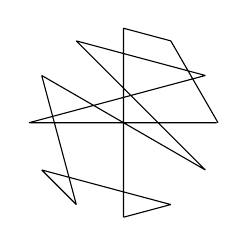
\begin{tikzpicture}[rotate=30*4,minimum height=0pt,inner sep=0pt,outer sep=0pt,scale=0.75]
			\foreach \x in {0,...,11} {\node (\x) at (90-30*\x:1.6) {};};
			
			\draw (4)--(5)--(7)--(1)--(6)--(3)--(8)--(2)--(11)--(0)--(9)--(10)--(4);
			\end{tikzpicture}
			%\vspace{-0.75cm}
			\centering
			
			%\caption*{\begin{center}{\footnotesize Espectro serial de la Suite Op. 25}\end{center}}
		\end{wrapfigure}
		Ahora se calcularán los espectros formados mediante todas las transformaciones del grupo generado por \{S,T,V,C\}. Volviendo a la representación mediante diagramas de reloj del apartado \ref{diagramas}, el problema es equivalente a averiguar cuántos diagramas distintos, sin números ni flechas, se pueden dibujar. La flecha indica lo transformado por V y C, mientras que los números indican lo transformado por S y T. Un diagrama sin estos dos elementos representa entonces todo un espectro serial. ¿Cuántos diagramas esencialmente distintos hay? De nuevo, por el lema de Burnside:	
		$$\#\text{Spec}=\#Orb=\frac{1}{|\text{D}_{n}\times\text{D}_{n}|}\sum_{\sigma\in\text{S}_n}|\text{Stab}(\sigma)|=\frac{1}{2n\cdot2n}\sum_{\sigma\in\text{S}_n}|\text{Stab}(\sigma)|$$
		
		En vez de expresar el sumatorio como ``para cada $\sigma$, el número de $\Psi$ que fijan $\sigma$'', se puede expresar como ``para cada $\Psi$, el número de $\sigma$ fijados por $\Psi$''. La fórmula queda de esta manera:
		$\#\text{Spec}=\frac{1}{4n^2}\sum_{\Psi\in\text{D}_{n}\times\text{D}_{n}}\text{Fij}(\Psi)$. Ahora hay que averiguar para cada elemento de $\text{D}_{n}\times\text{D}_{n}$ cuántas series estabiliza. Por ejemplo, trivialmente no hay permutaciones estables mediante C y R solamente.
		
		\subsection{Elementos estables mediante T}
		
		Los elementos estables mediante T$^\text{k}$ son a los que se aplica una rotación de $\uptheta_\text{k}=\frac{2\pi\text{k}}{n}$, para $1\leq\text{k}\leq n$, y quedan igual. Por tanto, los sumandos que aportan a la suma total son $\sum_{\text{k}=1}^{n}\text{Fij}(\uptheta_\text{k})$.
		
		Por otro lado, si $1\leq p,q\leq n$ y $gcd(n,p)=gcd(n,q)$ entonces $\text{Fij}(\uptheta_p)=\text{Fij}(\uptheta_q)$. Esto permite que se puedan agrupar los sumandos con igual máximo común divisor con respecto a $n$. Si $n=6$: 
		
		$\text{Fij}(\uptheta_\text{1})+\text{Fij}(\uptheta_\text{2})+\text{Fij}(\uptheta_\text{3})+\text{Fij}(\uptheta_\text{4})+\text{Fij}(\uptheta_\text{5})+\text{Fij}(\uptheta_\text{6})=%\hspace*{\hfill}
		\text{Fij}(\uptheta_\text{1})+\text{Fij}(\uptheta_\text{2})+\text{Fij}(\uptheta_\text{3})+\text{Fij}(\uptheta_\text{2})+\text{Fij}(\uptheta_\text{1})+\text{Fij}(\uptheta_\text{6})=%\hspace*{\hfill}
		2\cdot\text{Fij}(\uptheta_\text{1})+2\cdot\text{Fij}(\uptheta_\text{2})+1\cdot\text{Fij}(\uptheta_\text{3})+1\cdot\text{Fij}(\uptheta_\text{6})$
		
		Esos coeficientes son el número de \textit{totativos} de cada divisor $d$ de $n$, pero en orden contrario. Es decir, los totativos de $\frac{n}{d}$, que es el divisor opuesto a $d$. Los totativos de un número son los números menores que él y coprimos con él. La función que indica cuántos totativos tiene un número $n$ se llama la función $\varphi$ de Euler. Entonces $\sum_{\text{k}=1}^{n}\text{Fij}(\uptheta_\text{k})=\sum_{d|n}\left(\varphi(\frac{n}{d})\cdot\text{Fij}(\uptheta_d)\right)$.
		
		\begin{wrapfigure}{R}{0.15\textwidth}
			\vspace{0.5cm}
			\begin{tikzpicture}[minimum height=0pt,inner sep=0pt,outer sep=0pt,scale=0.75]
			\foreach \x in {0,...,5} {\node at (90-60*\x:2) {\x}; \node (\x) at (90-60*\x:1.6) {};};
			
			\draw [style=flechita] (0)--(3)--(2)--(4)--(1)--(5)--(0);
			\end{tikzpicture}
			
			\begin{tikzpicture}
			\draw[white] (-1.41,0) -- (0,0.25) -- (0,-1);
			\draw[style=flache] (0,0) -- node[right=7pt] {C} (0,-0.75);
			\end{tikzpicture}
			
			\begin{tikzpicture}[minimum height=0pt,inner sep=0pt,outer sep=0pt,scale=0.75]
			\foreach \x in {0,...,5} {\node at (90-60*\x:2) {\x}; \node (\x) at (90-60*\x:1.6) {};};
			
			\draw [style=flechita] (3)--(2)--(4)--(1)--(5)--(0)--(3);
			\end{tikzpicture}
			
			\begin{tikzpicture}
			\draw[white] (-1.41,0) -- (0,0.25) -- (0,-1);
			\draw[style=flache] (0,0) -- node[right=7pt] {V} (0,-0.75);
			\end{tikzpicture}
			
			\begin{tikzpicture}[minimum height=0pt,inner sep=0pt,outer sep=0pt,scale=0.75]
			\foreach \x in {0,...,5} {\node at (90-60*\x:2) {\x}; \node (\x) at (90-60*\x:1.6) {};};
			
			\draw [style=flechita] (3)--(0)--(5)--(1)--(4)--(2)--(3);
			\end{tikzpicture}
			
			\begin{tikzpicture}
			\draw[white] (-1.41,0) -- (0,0.25) -- (0,-1);
			\draw[style=flache] (0,0) -- node[right=7pt] {T$^3$} (0,-0.75);
			\end{tikzpicture}
			
			\begin{tikzpicture}[minimum height=0pt,inner sep=0pt,outer sep=0pt,scale=0.75]
			\foreach \x in {0,...,5} {\node at (90-60*\x:2) {\x}; \node (\x) at (90-60*\x:1.6) {};};
			
			\draw [style=flechita] (0)--(3)--(2)--(4)--(1)--(5)--(0);
			\end{tikzpicture}
			\vspace{-0.5cm}
		\end{wrapfigure}
		
		Para calcular $\text{Fij}(\uptheta_d)$ hay que analizar el método de construcción de diagramas invariantes respecto a una rotación. Estos diagramas deben tener varios loops iguales entre sí pero cada uno desde un punto distinto: desde cada múltiplo de $d$. El número de loops es, por tanto, $\frac{n}{d}$.
		
		Al construir uno de estos diagramas, se escoge la primera nota entre las $n$. Después, se escoge la segunda, pero no se puede escoger los vértices múltiplos de $d$ (de los que hay $\frac{n}{d}$), ya que van a ser el comienzo de los sucesivos loops. Hay entonces $n-\frac{n}{d}$ posibilidades. Después se escoge la tercera, pero sin escoger los múltiplos de $d$ ni los múltiplos de $d\ +$ la segunda posición. Hay $n - 2\cdot\frac{n}{d}$ posibilidades, y así sucesivamente hasta terminar el primer loop:
		$$n\left(n-\frac{n}{d}\right)\left(n-\frac{2n}{d}\right)\cdots\left(n-\frac{(d-1)n}{d}\right)=$$ 
		$$=n^d\left(1-\frac{1}{d}\right)\left(1-\frac{2}{d}\right)\cdots\left(1-\frac{d-1}{d}\right)=$$
		$$=n^d\left(\frac{d-1}{d}\right)\left(\frac{d-2}{d}\right)\cdots\left(\frac{1}{d}\right)=n^d\cdot\frac{(d-1)!}{d^{d-1}}\cdot\frac{d}{d}=\left(\frac{n}{d}\right)^d\cdot d!$$
		
		Para escoger el segundo loop, su primera nota debe caer en el conjunto de vértices múltiplos de $d$, y se puede escoger de $\varphi\left(\frac{n}{d}\right)$ formas. No son $\frac{n}{d}$ ya que tomar un vértice no coprimo implicaría que el polígono se cerraría antes de tiempo sin pasar por todos los vértices. Tras esto el polígono está totalmente determinado, y se puede formar de $\sum_{d|n}\left(\varphi^2(\frac{n}{d})\cdot\left(\frac{n}{d}\right)^d\cdot d!\right)$ maneras.
		
		Solamente para $n$ par hay un método más de construcción de polígono invariante mediante T, V y C a la vez, ya que al rotar $\frac{n}{2}$ el diagrama puede llegar con la orientación cambiada. A la derecha hay un ejemplo de ello. Esto puede ocurrir cuando entre dos notas haya un intervalo -- un salto -- de $\frac{n}{2}$.
		
		Primero se escoge la diagonal de entre $\frac{n}{2}$ posibilidades, con lo que queda dividida en dos la figura. De cada pareja de puntos antipodales se escoge el que irá primero en la ronda de elección. Esa elección para cada pareja opuesta se da de de $2^{\frac{n}{2}}$ formas. Tras lo cual se ordenan esos primeros miembros entre sí, de $\frac{n}{2}!$ formas. Esto lleva a las $\frac{n}{2}\cdot2^{\frac{n}{2}}\cdot\frac{n}{2}!$ formas de dibujar un polígono con las características buscadas.		
		
		\subsection{Elementos estables mediante I}
		
		Los elementos estables mediante I son aquellos que quedan invariantes mediante reflexiones. En este punto se ha de separar por paridad de $n$. 
		
		Para $n$ impar, existen $n$ reflexiones para cada uno de los ejes de simetría que pasan por cada vértice. Después, hay $n$ formas de escoger el primer vértice de la secuencia. Ahora hay $\frac{n-1}{2}$ parejas de vértices; se escoge los primeros miembros entre ellos de $2^{\frac{n-1}{2}}$ formas, tras lo cual éstos se ordenan de $\frac{n-1}{2}!$ formas. Esto da un resultado de  $n^2\cdot2^{\frac{n-1}{2}}\cdot\frac{n-1}{2}!$ polígonos invariantes.
		
		Para $n$ par se tienen dos simetrías: con ejes que pasan por vértices y con ejes que pasan por lados. De manera similar a la anterior, se escoge el eje, el primer vértice, los primeros miembros de las parejas de vértices y se ordenan. Para las simetrías con ejes que pasan por vértices, da un resultado de  $\frac{n^2}{2}\cdot2^{\frac{n}{2}}\cdot\left(\frac{n}{2}-1\right)!$. Para las simetrías con ejes que pasan por lados, da un resultado de $\frac{n^2}{2}\cdot2^{\frac{n}{2}-1}\cdot\frac{n}{2}!$.
		
		\subsection*{Suma completa}
		
		En resumen, estos son los numeradores $\sum_{\Psi\in\text{D}_{n}\times\text{D}_{n}}\text{Fij}(\Psi)$. El resultado final del número de diagramas posibles, o espectros seriales distintos, es dicho numerador entre $4n^2$, el tamaño del grupo. \footnote{Este apartado es una explicación detallada del artículo \cite{polygons}. La secuencia de números dada por las fórmulas demostradas se encuentra en la OEIS: \textit{https://oeis.org/A000940}}		
		\def\arraystretch{1.25}
		$$\begin{array}{c||c}
		&\textbf{\textit{n} IMPAR}\\\hline\hline
		\text{Rotación}&\sum_{d|n}\left(\varphi^2(\frac{n}{d})\cdot\left(\frac{n}{d}\right)^d\cdot d!\right)\\\hline
		\text{Reflexión}&n^2\cdot2^{\frac{n-1}{2}}\cdot\frac{n-1}{2}!\\\hline
		&\sum_{d|n}\left(\varphi^2(\frac{n}{d})\cdot\left(\frac{n}{d}\right)^d\cdot d!\right)+n^2\cdot2^{\frac{n-1}{2}}\cdot\frac{n-1}{2}!\\
		\end{array}$$
		
		$$\begin{array}{c||c}
		&\textbf{\textit{n} PAR}\\\hline\hline
		\text{Rotación}&\sum_{d|n}\left(\varphi^2(\frac{n}{d})\cdot\left(\frac{n}{d}\right)^d\cdot d!\right)\\\hline
		\text{Rotación con orientación}&\frac{n}{2}\cdot2^{\frac{n}{2}}\cdot\frac{n}{2}!\\\hline
		\text{Reflexión por vértices}&\frac{n^2}{2}\cdot2^{\frac{n}{2}}\cdot\left(\frac{n}{2}-1\right)!\\\hline
		\text{Reflexión por lados}&\frac{n^2}{2}\cdot2^{\frac{n}{2}-1}\cdot\frac{n}{2}!\\\hline
		&\sum_{d|n}\left(\varphi^2(\frac{n}{d})\cdot\left(\frac{n}{d}\right)^d\cdot d!\right)+\frac{n(n+6)}{4}\cdot2^{\frac{n}{2}}\cdot\frac{n}{2}!\\
		\end{array}$$
		\def\arraystretch{1}
		
	\section{Medefonismo, monofonismo y difonismo}
	\label{monodi}
		Con $n=0$ se da el caso de medefonismo. El grupo simétrico de orden 0 tiene $0!=1$ elemento. Por tanto, hay una sola posible serie, $\sigma$, que es la que no tiene ninguna nota. El medefonismo es comúnmente llamado silencio.
		
		$$\sigma=\left(\begin{matrix}\\\end{matrix}\right)
		\hspace{5cm}
		\begin{array}{l||r}
		&\\
		\hline
		\hline
		&\\
		\hline
		&
		\end{array}$$
	
		Con $n=1$ se da el caso de monofonismo. Con solamente una posible nota, el grupo simétrico de orden 1 tiene $1!=1$ elemento. Por tanto, hay una sola posible serie, $\sigma_0$, que es igual a su inversa, a su retrogradación y a su retrogradación inversa:
		$$\sigma_0=\left(\begin{matrix}0\\0\end{matrix}\right)
		\hspace{3cm}
		\begin{array}{l|c|r}
			&\text{I}_{0}&\\
			\hline
			\text{T}_{0}&0&\text{R}_{0}\\
			\hline
			&\text{IR}_{0}&\\
			\hline
			&\text{RI}_{0}&
		\end{array}$$
	
		Con $n=2$ se da el caso de difonismo. Tiene dos posibles notas, así que su grupo simétrico, el de orden 2, tiene $2!=2$ elementos. Por tanto, hay dos series distintas, $\sigma_0$ y $\sigma_1$. Se puede observar que ambas pertenecen al mismo espectro serial, dado que $\sigma_1=\text{T}^1(\sigma_0)$. Además, al igual que en el monofonismo, ambas coinciden con sus inversas, incumpliendo la regla general para $n>2$ probada en el apartado \ref{inversano}.
		$$\sigma_0=\left(\begin{matrix}0&1\\0&1\end{matrix}\right)
		\hspace{2cm}
		\begin{array}{l|cc|r}
			&\text{I}_{0}&\text{I}_{1}&\\
			\hline
			\text{T}_{0}&0&1&\text{R}_{0}\\
			\text{T}_{1}&1&0&\text{R}_{1}\\
			\hline
			&\text{IR}_{0}&\text{IR}_{1}&\\
			\hline
			&\text{RI}_{0}&\text{RI}_{1}&
		\end{array}
		\hspace{2cm}
		\sigma_1=\left(\begin{matrix}0&1\\1&0\end{matrix}\right)$$